\documentclass[11pt,a4paper]{article}
\usepackage[utf8]{inputenc}
\usepackage[T1]{fontenc}
\usepackage[english]{babel}
\usepackage{geometry}
\geometry{margin=2cm}
\usepackage{graphicx}
\usepackage{hyperref}
\usepackage{xcolor}
\usepackage{amsmath}
\usepackage{booktabs}
\usepackage{longtable}
\usepackage{fancyhdr}
\usepackage{tikz}
\usetikzlibrary{shapes,arrows,positioning}

\pagestyle{fancy}
\fancyhf{}
\rhead{Quantum Testing Agent — Vultr Agent Rush}
\lhead{\thepage}

\definecolor{codebg}{rgb}{0.95,0.95,0.95}
% listings no disponible: usar verbatim para código
% \lstset{...}

\title{\textbf{Quantum Testing Agent}\\
\large Agente de pruebas cuánticas aislado en sandbox Docker\\
\large para Vultr: Agent Rush Hackathon}
\author{Jesús León Porras\\
\texttt{jalp17@github}}
\date{8 de noviembre de 2026}

\begin{document}

\maketitle

\begin{abstract}
Este documento presenta el diseño, arquitectura y plan de implementación del
\textbf{Quantum Testing Agent}, un agente web que ejecuta pruebas de circuitos y
simulaciones cuánticas dentro de un sandbox Docker aislado en Vultr. El proyecto
participa en el desafío \textit{Blast Radius Zero} del hackathon Vultr: Agent Rush
(lablab.ai $\times$ Vultr, 3--8 nov 2026). El agente planifica la prueba mediante
un LLM (Vultr Serverless Inference), genera código en el framework solicitado
(Qiskit, PennyLane, Cirq, Azure Quantum), lo ejecuta en un contenedor desechable
con límites de recursos y devuelve un resultado verificable. La contención es
obligatoria: el sandbox absorbe fallos (bucles infinitos, comandos destructivos)
sin comprometer el host ni el backend.
\end{abstract}

\tableofcontents
\newpage

% ============================================================
\section{Contexto del hackathon}

El hackathon \textbf{Vultr: Agent Rush} es un evento híbrido organizado por
lablab.ai y Vultr, con fase de construcción online del 3 al 8 de noviembre de
2026 y fase presencial el 8 de noviembre en Salt Lake City, UT.

\subsection{Objetivo}

Construir un agente de IA que realice trabajo real --- escribir y ejecutar código
o operar un navegador real --- con cada acción contenida dentro de un sandbox
aislado en Vultr. El sistema actúa como capa de control centralizada: planifica
la tarea, la despacha a un entorno de ejecución aislado y devuelve salida
verificable.

\subsection{Desafío elegido: Blast Radius Zero}

El agente web ejecuta trabajo real (código cuántico) dentro de un sandbox aislado
en Vultr. Patrones de ejecución:

\begin{itemize}
    \item \textbf{Pattern A (Sandboxed code execution):} usuario pide $\rightarrow$
    modelo escribe código $\rightarrow$ código se ejecuta en contenedor $\rightarrow$
    salida real retorna $\rightarrow$ modelo explica el resultado.
    \item \textbf{Pattern B (Sandboxed browser use):} objetivo $\rightarrow$ plan
    $\rightarrow$ Playwright en contenedor $\rightarrow$ capturas $\rightarrow$
    visión verifica $\rightarrow$ aprobación humana.
\end{itemize}

Este proyecto se enfoca en el \textbf{Pattern A}, que es el núcleo del valor.

\subsection{Stack tecnológico requerido}

\begin{table}[h]
\centering
\begin{tabular}{lll}
\toprule
\textbf{Componente} & \textbf{Detalle} & \textbf{Requerido} \\
\midrule
Vultr Cloud Compute & VM backend, capa de control & Sí (ambos) \\
Vultr Serverless Inference & OpenAI-compatible, \texttt{api.vultrinference.com/v1} & C1: Sí, C2: No \\
Agent sandboxing & Docker, OpenSandbox, gVisor, E2B, Microsandbox & C1: Sí \\
Vultr API & Instancias desechables por tarea & Opcional \\
GPUs de Vultr & No disponibles en este evento & --- \\
\bottomrule
\end{tabular}
\caption{Stack tecnológico del hackathon}
\end{table}

\subsection{Entregables requeridos}

\begin{enumerate}
    \item Repositorio público de GitHub con setup y documentación.
    \item Backend desplegado en VM de Vultr, LLM vía Vultr Serverless Inference.
    \item URL pública de demo (experiencia con estilo de producto).
    \item Vídeo de demo grabado incluyendo un momento de contención.
    \item Explicación clara de la arquitectura y el caso de uso.
    \item Envío oficial en lablab.ai.
\end{enumerate}

\subsection{Criterios de juzgamiento (1--5 cada uno)}

\begin{enumerate}
    \item Application of Technology
    \item Presentation
    \item Business Value
    \item Originality
\end{enumerate}

\textbf{Advertencia:} falta vídeo, enlace de demo o GitHub $\rightarrow$ calificación
de 1 en Presentación. Tres de cuatro criterios se hunden por falta de paperwork.

% ============================================================
\section{Descripción del proyecto}

\subsection{Qué es}

El \textbf{Quantum Testing Agent} es un agente web que recibe una especificación
de circuito cuántico, planifica la prueba mediante un LLM (Vultr Serverless
Inference), genera código en el framework elegido (Qiskit, PennyLane, Cirq, Azure
Quantum), lo ejecuta dentro de un sandbox Docker aislado en una VM de Vultr y
devuelve un resultado verificable.

\subsection{Problema}

Probar circuitos y simulaciones cuánticas es riesgoso: el código puede ser
arbitrario, contener bucles infinitos, comandos destructivos o consumir recursos
sin límite. Ejecutarlo directamente en el host o en el backend compromete la
seguridad del sistema. Además, los frameworks cuánticos son heterogéneos
(Qiskit/IBM, PennyLane/AWS, Cirq/Google, Azure Quantum/Microsoft), lo que
complica la compatibilidad.

\subsection{Solución}

Un agente que \textbf{aisla cada ejecución} en un contenedor Docker desechable
con límites de CPU, memoria y tiempo. El sandbox se destruye tras cada tarea,
garantizando que ningún código cuántico toque el host ni el backend. La
contención se demuestra en el vídeo de demo: el sandbox absorbe un bucle
infinito o un comando \texttt{rm -rf} y el sistema permanece intacto.

\subsection{Compatibilidad}

\begin{itemize}
    \item \textbf{Frameworks:} Qiskit (IBM), PennyLane (AWS Braket), Cirq
    (Google), Azure Quantum (Microsoft).
    \item \textbf{Hardware:} simulador CPU local como fallback (compatible con
    NVIDIA CUDA-Q y AMD ROCm); backends remotos opcionales para hardware cuántico
    real.
    \item \textbf{Nubes:} IBM Quantum, AWS Braket, Azure Quantum, Google Quantum.
\end{itemize}

% ============================================================
\section{Arquitectura}

\subsection{Modelo C4 -- Nivel 1: Contexto}

\begin{center}
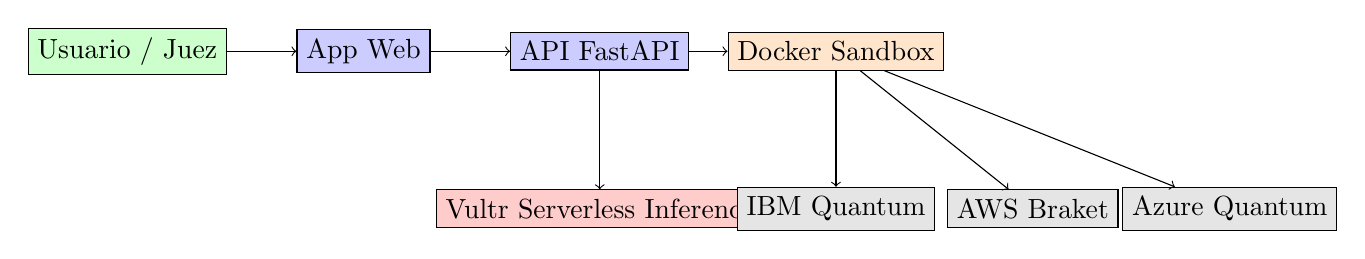
\begin{tikzpicture}[node distance=2cm, auto]
    \node[draw, rectangle, fill=green!20] (user) {Usuario / Juez};
    \node[draw, rectangle, fill=blue!20, right of=user, node distance=3cm] (web) {App Web};
    \node[draw, rectangle, fill=blue!20, right of=web, node distance=3cm] (api) {API FastAPI};
    \node[draw, rectangle, fill=red!20, below of=api, node distance=2cm] (inf) {Vultr Serverless Inference};
    \node[draw, rectangle, fill=orange!20, right of=api, node distance=3cm] (sandbox) {Docker Sandbox};
    \node[draw, rectangle, fill=gray!20, below of=sandbox, node distance=2cm] (ibm) {IBM Quantum};
    \node[draw, rectangle, fill=gray!20, right of=ibm, node distance=2.5cm] (aws) {AWS Braket};
    \node[draw, rectangle, fill=gray!20, right of=aws, node distance=2.5cm] (azure) {Azure Quantum};

    \draw[->] (user) -- (web);
    \draw[->] (web) -- (api);
    \draw[->] (api) -- (inf);
    \draw[->] (api) -- (sandbox);
    \draw[->] (sandbox) -- (ibm);
    \draw[->] (sandbox) -- (aws);
    \draw[->] (sandbox) -- (azure);
\end{tikzpicture}
\end{center}

\subsection{Modelo C4 -- Nivel 2: Contenedores}

\begin{table}[h]
\centering
\begin{tabular}{lll}
\toprule
\textbf{Contenedor} & \textbf{Responsabilidad} & \textbf{Stack} \\
\midrule
App Web & UI de entrada y visualización & HTML/JS \\
API FastAPI & Endpoints REST: crear tarea, estado, resultado & Python, FastAPI, uvicorn \\
Agente Orquestador & Descompone tarea, genera código, verifica & Python, LLM vía Vultr \\
Docker Engine & Levanta/destruye contenedores aislados & Docker, cgroups \\
Sandbox por tarea & Ejecuta código cuántico con límites & python:3.11-slim \\
\bottomrule
\end{tabular}
\caption{Contenedores del sistema}
\end{table}

\subsection{Modelo C4 -- Nivel 3: Componentes (backend)}

\begin{table}[h]
\centering
\begin{tabular}{llll}
\toprule
\textbf{Componente} & \textbf{Qué hace} & \textbf{Entrada} & \textbf{Salida} \\
\midrule
Task Planner & Descompone especificación en pasos & Especificación & Lista de pasos \\
Code Generator & Escribe código de prueba & Paso + framework & Archivo .py \\
Sandbox Runner & Levanta contenedor, límites, ejecuta, destruye & Archivo .py & Salida + código de salida \\
Result Verifier & Evalúa validez y contención & Salida cruda & Resultado verificable \\
Hardware Abstraction & Normaliza llamadas a backends & Resultado & Datos unificados \\
\bottomrule
\end{tabular}
\caption{Componentes del backend}
\end{table}

\subsection{Despliegue}

\begin{itemize}
    \item \textbf{VM Vultr:} backend FastAPI + Docker Engine como capa de control.
    \item \textbf{Vultr Serverless Inference:} llamadas LLM (planificación, generación, explicación).
    \item \textbf{Backends remotos:} IBM Quantum, AWS Braket, Azure Quantum (opcionales, configurables vía variables de entorno).
    \item \textbf{Simulador CPU local:} fallback sin dependencias externas.
\end{itemize}

% ============================================================
\section{Flujo de trabajo (UML)}

\subsection{Diagrama de secuencia}

\begin{enumerate}
    \item Usuario especifica circuito + framework + shots en la web.
    \item Web envía \texttt{POST /tasks} a la API FastAPI.
    \item API crea la tarea y llama al orquestador.
    \item Orquestador pide plan de descomposición al LLM (Vultr Serverless Inference).
    \item LLM devuelve pasos de prueba.
    \item Orquestador genera código de prueba en el framework elegido.
    \item Sandbox Runner levanta contenedor Docker aislado con límites.
    \item Código cuántico se ejecuta dentro del sandbox.
    \item Sandbox devuelve salida + código de salida.
    \item Contenedor se destruye (disciplina de ciclo de vida).
    \item Result Verifier verifica salida y contención.
    \item Resultado verificable se devuelve a la UI web.
\end{enumerate}

\subsection{Flujo de estados de la tarea}

\begin{center}
\texttt{creada} $\rightarrow$ \texttt{planificada} $\rightarrow$ \texttt{codigo\_generado}
$\rightarrow$ \texttt{sandbox\_levantado} $\rightarrow$ \texttt{ejecutando} \\
$\rightarrow$ \texttt{completada} / \texttt{fallida\_ejecucion} \\
$\rightarrow$ \texttt{verificada} $\rightarrow$ \texttt{resultado\_listo}
\end{center}

\subsection{Reglas de contención (obligatorio)}

\begin{enumerate}
    \item \textbf{Aislamiento de procesos:} el código cuántico nunca toca el host ni el runtime de la API.
    \item \textbf{Higiene de secretos:} ninguna API key dentro del sandbox; credenciales solo en el backend.
    \item \textbf{Límites de recursos:} tope de CPU, memoria y tiempo por contenedor (ej. 60 s, 512 MB).
    \item \textbf{Disciplina de ciclo de vida:} el contenedor se destruye tras cada tarea, exitoso o fallido.
    \item \textbf{Momento de contención en demo:} el vídeo muestra el sandbox absorbiendo un \texttt{rm -rf}, bucle infinito o circuito hostil sin comprometer el sistema.
\end{enumerate}

% ============================================================
\section{Decisión de arquitectura (ADR-0001)}

\subsection{Contexto}

El proyecto participa en Vultr: Agent Rush (3--8 nov 2026). Desafío: Blast Radius
Zero. Requisitos: VM Vultr como backend, Vultr Serverless Inference para LLM,
Docker sandbox, sin GPUs disponibles.

\subsection{Alternativas evaluadas}

\begin{table}[h]
\centering
\begin{tabular}{lp{4cm}p{4cm}p{3cm}}
\toprule
\textbf{Alt.} & \textbf{Descripción} & \textbf{Ventajas} & \textbf{Desventajas} \\
\midrule
A1 & Simulador CPU local & Sin dependencias externas & Limitado a CPU, no demuestra multi-nube \\
A2 & Backends remotos (IBM/AWS/Azure) & Hardware cuántico real & Colas, costos, credenciales \\
A3 & Híbrido: CPU fallback + remotos & Demo robusto + multi-nube & Mayor complejidad \\
A4 & GPUs locales (NVIDIA/AMD) & Aceleración hardware & Inviable: sin GPUs en Vultr \\
\bottomrule
\end{tabular}
\caption{Alternativas de arquitectura}
\end{table}

\subsection{Decisión}

Se adopta la \textbf{alternativa A3 (híbrida)}: simulador CPU local como fallback
garantizado + adaptadores para IBM/AWS/Azure/Google como backends remotos
opcionales. Toda la inferencia del agente usa Vultr Serverless Inference. El
sandbox es un contenedor Docker desechable con límites, destruido tras cada tarea.

\subsection{Consecuencias}

\begin{itemize}
    \item \textbf{Positivas:} demo robusto sin depender de colas externas; cumple
    requisitos del hackathon; contención verificable.
    \item \textbf{Negativas:} simulador CPU más lento que GPU; limitar demo a
    circuitos pequeños ($\leq$ 20 qubits); complejidad de adaptadores.
\end{itemize}

% ============================================================
\section{Implementación}

\subsection{Estructura del proyecto}

\begin{verbatim}
quantum-testing-agent/
├── app/
│   ├── __init__.py
│   ├── main.py              # FastAPI: /health, /tasks, /tasks/{id}, /
│   ├── models.py            # CircuitSpec, TaskResult, TaskStatus, Framework
│   ├── store.py             # Almacenamiento en memoria
│   ├── orchestrator.py      # Planificación LLM + generación de código
│   ├── sandbox.py           # Docker sandbox con límites y destroy
│   └── backend_adapters.py  # Qiskit, PennyLane, Cirq, Azure, CPU local
├── tests/
│   ├── test_basic.py        # Tests de orquestador y store
│   └── test_api.py          # Tests de API (health, tasks, contención)
├── docs/
│   ├── C4.md
│   ├── workflow.md
│   ├── ADR/0001-*.md
│   └── demo-script.md
├── requirements.txt
├── .env.example
├── Dockerfile
├── docker-compose.yml
├── README.md
└── AGENTS.md
\end{verbatim}

\subsection{Endpoints de la API}

\begin{table}[h]
\centering
\begin{tabular}{lll}
\toprule
\textbf{Método} & \textbf{Ruta} & \textbf{Descripción} \\
\midrule
GET & \texttt{/health} & Estado del servicio y sandbox \\
POST & \texttt{/tasks} & Crear y ejecutar tarea de prueba cuántica \\
GET & \texttt{/tasks/\{id\}} & Estado y resultado de la tarea \\
GET & \texttt{/} & UI web de demo \\
\bottomrule
\end{tabular}
\caption{Endpoints de la API}
\end{table}

\subsection{Tests}

\begin{table}[h]
\centering
\begin{tabular}{ll}
\toprule
\textbf{Test} & \textbf{Qué verifica} \\
\midrule
test\_health & Endpoint /health responde OK \\
test\_create\_task & POST /tasks crea y ejecuta tarea \\
test\_create\_task\_containment & Sandbox contiene código hostil \\
test\_plan\_task & Orquestador genera plan \\
test\_generate\_code & Genera código por framework \\
test\_store\_and\_get & Almacenamiento y recuperación \\
\bottomrule
\end{tabular}
\caption{6 tests, todos pasando}
\end{table}

% ============================================================
\section{Guion de demo}

\subsection{Objetivo}

Demostrar un agente web que prueba circuitos cuánticos de forma aislada y
verificable en Vultr, cumpliendo el desafío Blast Radius Zero. Duración
$\leq$ 5 minutos. Debe incluir un \textbf{momento de contención}.

\subsection{Guion paso a paso}

\begin{table}[h]
\centering
\begin{tabular}{clp{6cm}c}
\toprule
\# & Paso & Qué se muestra & Tiempo \\
\midrule
1 & Apertura & Problema: probar código cuántico es riesgoso; solución: sandbox aislado & 30 s \\
2 & Entrada & Usuario escribe circuito de 3 qubits + Hadamard + CNOT en Qiskit & 30 s \\
3 & Planificación & Agente (Vultr Inference) descompone en pasos, muestra plan & 30 s \\
4 & Generación & Código Qiskit generado, mostrado brevemente & 20 s \\
5 & Ejecución & Contenedor Docker levantado con límites, código ejecutado & 45 s \\
6 & Resultado & Estados de medida y histogramas verificables & 30 s \\
7 & Contención & Código hostil (bucle infinito) $\rightarrow$ sandbox lo absorbe y destruye & 60 s \\
8 & Multi-framework & Selección de PennyLane/Cirq, prueba repetida & 30 s \\
9 & Cierre & Resumen de arquitectura + llamada a acción & 45 s \\
\bottomrule
\end{tabular}
\caption{Guion de demo ($\approx$ 4 min 30 s)}
\end{table}

\subsection{Momento de contención (clave para el vídeo)}

\begin{itemize}
    \item \textbf{Entrada hostil:} código con \texttt{while True: pass} o
    \texttt{os.system("rm -rf /tmp/test")}.
    \item \textbf{Comportamiento:} el contenedor alcanza el límite de tiempo/memoria,
    Docker lo mata, el entorno se destruye, la API responde con
    \texttt{containment: true}.
    \item \textbf{Evidencia en vídeo:} terminal del backend registrando la
    destrucción del contenedor + web mostrando estado seguro.
\end{itemize}

\subsection{Requisitos técnicos para la demo}

\begin{table}[h]
\centering
\begin{tabular}{ll}
\toprule
\textbf{Requisito} & \textbf{Detalle} \\
\midrule
Backend desplegado & VM de Vultr con FastAPI + Docker, URL pública \\
LLM & Vultr Serverless Inference \\
Frameworks en Docker & Qiskit, PennyLane (Cirq, Azure opcionales) \\
Límites de sandbox & 60 s CPU, 512 MB memoria, red desactivada \\
Repo público & GitHub con README, setup, docs, guion de demo \\
Vídeo & $\leq$ 5 min, MP4, $\leq$ 300 MB, con contención \\
\bottomrule
\end{tabular}
\caption{Requisitos técnicos}
\end{table}

% ============================================================
\section{Próximos pasos}

\begin{enumerate}
    \item Configurar \texttt{.env} con \texttt{VULTR\_API\_KEY} y
    \texttt{VULTR\_INFERENCE\_URL}.
    \item Desplegar en VM de Vultr: \texttt{docker-compose up -d}.
    \item Grabar vídeo de demo ($\leq$ 5 min) con momento de contención.
    \item Subir repo a GitHub público y enviar en lablab.ai.
    \item Verificar que la URL de demo es accesible públicamente.
\end{enumerate}

% ============================================================
\section{Referencias}

\begin{itemize}
    \item Vultr: Agent Rush Hackathon --- \url{https://lablab.ai/ai-hackathons/vultr-hackathon}
    \item Vultr Community --- \url{https://community.vultr.com/e/vultr-agent-rush-hackathon}
    \item Luma --- \url{https://luma.com/lablab-8d5a}
    \item Repositorio GitHub --- \url{https://github.com/jalp17/quantum-testing-agent}
\end{itemize}

\end{document}
